\documentclass[]{article}
\usepackage{lmodern}
\usepackage{amssymb,amsmath}
\usepackage{ifxetex,ifluatex}
\usepackage{fixltx2e} % provides \textsubscript
\ifnum 0\ifxetex 1\fi\ifluatex 1\fi=0 % if pdftex
  \usepackage[T1]{fontenc}
  \usepackage[utf8]{inputenc}
\else % if luatex or xelatex
  \ifxetex
    \usepackage{mathspec}
  \else
    \usepackage{fontspec}
  \fi
  \defaultfontfeatures{Ligatures=TeX,Scale=MatchLowercase}
\fi
% use upquote if available, for straight quotes in verbatim environments
\IfFileExists{upquote.sty}{\usepackage{upquote}}{}
% use microtype if available
\IfFileExists{microtype.sty}{%
\usepackage{microtype}
\UseMicrotypeSet[protrusion]{basicmath} % disable protrusion for tt fonts
}{}
\usepackage[margin=1in]{geometry}
\usepackage{hyperref}
\hypersetup{unicode=true,
            pdftitle={slurm},
            pdfauthor={Jakub Widawski},
            pdfborder={0 0 0},
            breaklinks=true}
\urlstyle{same}  % don't use monospace font for urls
\usepackage{color}
\usepackage{fancyvrb}
\newcommand{\VerbBar}{|}
\newcommand{\VERB}{\Verb[commandchars=\\\{\}]}
\DefineVerbatimEnvironment{Highlighting}{Verbatim}{commandchars=\\\{\}}
% Add ',fontsize=\small' for more characters per line
\usepackage{framed}
\definecolor{shadecolor}{RGB}{248,248,248}
\newenvironment{Shaded}{\begin{snugshade}}{\end{snugshade}}
\newcommand{\AlertTok}[1]{\textcolor[rgb]{0.94,0.16,0.16}{#1}}
\newcommand{\AnnotationTok}[1]{\textcolor[rgb]{0.56,0.35,0.01}{\textbf{\textit{#1}}}}
\newcommand{\AttributeTok}[1]{\textcolor[rgb]{0.77,0.63,0.00}{#1}}
\newcommand{\BaseNTok}[1]{\textcolor[rgb]{0.00,0.00,0.81}{#1}}
\newcommand{\BuiltInTok}[1]{#1}
\newcommand{\CharTok}[1]{\textcolor[rgb]{0.31,0.60,0.02}{#1}}
\newcommand{\CommentTok}[1]{\textcolor[rgb]{0.56,0.35,0.01}{\textit{#1}}}
\newcommand{\CommentVarTok}[1]{\textcolor[rgb]{0.56,0.35,0.01}{\textbf{\textit{#1}}}}
\newcommand{\ConstantTok}[1]{\textcolor[rgb]{0.00,0.00,0.00}{#1}}
\newcommand{\ControlFlowTok}[1]{\textcolor[rgb]{0.13,0.29,0.53}{\textbf{#1}}}
\newcommand{\DataTypeTok}[1]{\textcolor[rgb]{0.13,0.29,0.53}{#1}}
\newcommand{\DecValTok}[1]{\textcolor[rgb]{0.00,0.00,0.81}{#1}}
\newcommand{\DocumentationTok}[1]{\textcolor[rgb]{0.56,0.35,0.01}{\textbf{\textit{#1}}}}
\newcommand{\ErrorTok}[1]{\textcolor[rgb]{0.64,0.00,0.00}{\textbf{#1}}}
\newcommand{\ExtensionTok}[1]{#1}
\newcommand{\FloatTok}[1]{\textcolor[rgb]{0.00,0.00,0.81}{#1}}
\newcommand{\FunctionTok}[1]{\textcolor[rgb]{0.00,0.00,0.00}{#1}}
\newcommand{\ImportTok}[1]{#1}
\newcommand{\InformationTok}[1]{\textcolor[rgb]{0.56,0.35,0.01}{\textbf{\textit{#1}}}}
\newcommand{\KeywordTok}[1]{\textcolor[rgb]{0.13,0.29,0.53}{\textbf{#1}}}
\newcommand{\NormalTok}[1]{#1}
\newcommand{\OperatorTok}[1]{\textcolor[rgb]{0.81,0.36,0.00}{\textbf{#1}}}
\newcommand{\OtherTok}[1]{\textcolor[rgb]{0.56,0.35,0.01}{#1}}
\newcommand{\PreprocessorTok}[1]{\textcolor[rgb]{0.56,0.35,0.01}{\textit{#1}}}
\newcommand{\RegionMarkerTok}[1]{#1}
\newcommand{\SpecialCharTok}[1]{\textcolor[rgb]{0.00,0.00,0.00}{#1}}
\newcommand{\SpecialStringTok}[1]{\textcolor[rgb]{0.31,0.60,0.02}{#1}}
\newcommand{\StringTok}[1]{\textcolor[rgb]{0.31,0.60,0.02}{#1}}
\newcommand{\VariableTok}[1]{\textcolor[rgb]{0.00,0.00,0.00}{#1}}
\newcommand{\VerbatimStringTok}[1]{\textcolor[rgb]{0.31,0.60,0.02}{#1}}
\newcommand{\WarningTok}[1]{\textcolor[rgb]{0.56,0.35,0.01}{\textbf{\textit{#1}}}}
\usepackage{graphicx}
% grffile has become a legacy package: https://ctan.org/pkg/grffile
\IfFileExists{grffile.sty}{%
\usepackage{grffile}
}{}
\makeatletter
\def\maxwidth{\ifdim\Gin@nat@width>\linewidth\linewidth\else\Gin@nat@width\fi}
\def\maxheight{\ifdim\Gin@nat@height>\textheight\textheight\else\Gin@nat@height\fi}
\makeatother
% Scale images if necessary, so that they will not overflow the page
% margins by default, and it is still possible to overwrite the defaults
% using explicit options in \includegraphics[width, height, ...]{}
\setkeys{Gin}{width=\maxwidth,height=\maxheight,keepaspectratio}
\IfFileExists{parskip.sty}{%
\usepackage{parskip}
}{% else
\setlength{\parindent}{0pt}
\setlength{\parskip}{6pt plus 2pt minus 1pt}
}
\setlength{\emergencystretch}{3em}  % prevent overfull lines
\providecommand{\tightlist}{%
  \setlength{\itemsep}{0pt}\setlength{\parskip}{0pt}}
\setcounter{secnumdepth}{0}
% Redefines (sub)paragraphs to behave more like sections
\ifx\paragraph\undefined\else
\let\oldparagraph\paragraph
\renewcommand{\paragraph}[1]{\oldparagraph{#1}\mbox{}}
\fi
\ifx\subparagraph\undefined\else
\let\oldsubparagraph\subparagraph
\renewcommand{\subparagraph}[1]{\oldsubparagraph{#1}\mbox{}}
\fi

%%% Use protect on footnotes to avoid problems with footnotes in titles
\let\rmarkdownfootnote\footnote%
\def\footnote{\protect\rmarkdownfootnote}

%%% Change title format to be more compact
\usepackage{titling}

% Create subtitle command for use in maketitle
\providecommand{\subtitle}[1]{
  \posttitle{
    \begin{center}\large#1\end{center}
    }
}

\setlength{\droptitle}{-2em}

  \title{slurm}
    \pretitle{\vspace{\droptitle}\centering\huge}
  \posttitle{\par}
    \author{Jakub Widawski}
    \preauthor{\centering\large\emph}
  \postauthor{\par}
      \predate{\centering\large\emph}
  \postdate{\par}
    \date{1/21/2020}


\begin{document}
\maketitle

\hypertarget{slurm-assignment}{%
\section{SLURM ASSIGNMENT}\label{slurm-assignment}}

\hypertarget{excercise-1}{%
\subsection{Excercise 1}\label{excercise-1}}

Write a submit script from scratch -- The script should use the
following parameters: • Uses 1 node from the research.q queue • Creates
a file (called text.txt with content: ``I have written a submit script''
• Sleeps for 30 seconds • Lists the contents of the folder

\begin{Shaded}
\begin{Highlighting}[]
\CommentTok{\#!/bin/bash}
\CommentTok{\#SBATCH {-}{-}job{-}name=kuba}
\CommentTok{\#SBATCH {-}{-}partition=research.q}
\CommentTok{\#SBATCH {-}{-}nodes=1}
\CommentTok{\#SBATCH {-}{-}output=kuba\_slurm\_out}

\CommentTok{\# write string to file}
\BuiltInTok{echo} \StringTok{"I have submitted a script"} \OperatorTok{>}\NormalTok{ text.txt}

\CommentTok{\# sleep 30 seconds}
\FunctionTok{sleep}\NormalTok{ 30 }

\CommentTok{\# list contents of folder}
\FunctionTok{ls}
\end{Highlighting}
\end{Shaded}

Submit the same job from the command line (i.e.~all sbatch options
should be added to the command line together with a script file)

\begin{Shaded}
\begin{Highlighting}[]
\ExtensionTok{sbatch}\NormalTok{ slurm\_file {-}{-}job{-}name=kuba {-}{-}partition=research.q \textbackslash{}}
\NormalTok{                  {-}{-}nodes=1 {-}{-}output=kuba\_slurm\_out}
\end{Highlighting}
\end{Shaded}

Do the same without using the script file (i.e.~adding a --wrap option)

\begin{Shaded}
\begin{Highlighting}[]
\ExtensionTok{sbatch}\NormalTok{ {-}{-}wrap=}\StringTok{"echo \textquotesingle{}I have submitted a script\textquotesingle{} > text.txt;sleep 30;ls;"}\NormalTok{ {-}{-}job{-}name=kuba {-}{-}partition=research.q \textbackslash{}}
\NormalTok{                  {-}{-}nodes=1 {-}{-}output=kuba\_slurm\_out}
\end{Highlighting}
\end{Shaded}

\hypertarget{excercise-2}{%
\subsection{Excercise 2}\label{excercise-2}}

We want to sort several text files (names\_0.txt\ldots names\_4.txt).
Write a solution that uses SLURM job arrays. (Hint: use the sort command
from Linux to build your solution) Useful SLURM variables: -
SLURM\_ARRAY\_JOB\_ID set to the job ID for an array job. -
SLURM\_ARRAY\_TASK\_ID set to the task ID inside an array job. -
SLURM\_ARRAY\_TASK\_MAX/SLURM\_ARRAY\_TASK\_MIN maximum and minimum task
IDs in an array job.

\begin{Shaded}
\begin{Highlighting}[]
\CommentTok{\#!/bin/bash}
\CommentTok{\#SBATCH {-}{-}job{-}name=kuba\_exc2}
\CommentTok{\#SBATCH {-}{-}partition=research.q}
\CommentTok{\#SBATCH {-}{-}array=0{-}4}
\CommentTok{\#SBATCH {-}{-}output=kuba\_array.out}
\BuiltInTok{echo} \VariableTok{$(}\FunctionTok{sort}\NormalTok{ names\_}\VariableTok{$SLURM\_ARRAY\_TASK\_ID}\NormalTok{.txt}\VariableTok{)} \OperatorTok{>}\NormalTok{ names\_}\VariableTok{$SLURM\_ARRAY\_TASK\_ID}\NormalTok{.txt   }
\end{Highlighting}
\end{Shaded}

\hypertarget{exercise-3}{%
\subsection{Exercise 3}\label{exercise-3}}

Modify Job4 and turn it into an array job. When does Job5 start now?

Job5 starts after all the array jobs from job4 have been completed or
terminated due to the defined depedency (afterany: \$jid4)

It will start relatively quicker due to job4 being modified into an
array job which splits the tasks in the file.

job4.slurm

\begin{Shaded}
\begin{Highlighting}[]
\CommentTok{\#!/bin/bash}
\CommentTok{\#SBATCH {-}{-}job{-}name=basic{-}job}
\CommentTok{\#SBATCH {-}{-}output=basic{-}job{-}output}
\CommentTok{\#SBATCH {-}{-}partition=research.q}
\CommentTok{\#SBATCH {-}{-}nodelist=aolin23,aolin24}
\CommentTok{\#SBATCH {-}{-}array=0{-}4}
\CommentTok{\# print initial date and time}
\BuiltInTok{echo} \StringTok{"Start JOB 4 at }\VariableTok{$(}\FunctionTok{date}\VariableTok{)}\StringTok{"}
\BuiltInTok{echo} \StringTok{"{-}{-}{-}{-}{-}{-}{-}{-}{-}{-}{-}{-}{-}{-}{-}{-}{-}{-}{-}{-}{-}{-}{-}{-}{-}"}
\CommentTok{\# \# print name of host}
\FunctionTok{hostname}
\BuiltInTok{echo} \StringTok{"{-}{-}{-}{-}{-}{-}{-}{-}{-}{-}{-}{-}{-}{-}{-}{-}{-}{-}{-}{-}{-}{-}{-}{-}{-}"}
\CommentTok{\# sleep 20 seconds}
\FunctionTok{sleep}\NormalTok{ 20}
\CommentTok{\# print initial date and time}
\BuiltInTok{echo} \StringTok{"End JOB 4 at }\VariableTok{$(}\FunctionTok{date}\VariableTok{)}\StringTok{"}
\end{Highlighting}
\end{Shaded}

\hypertarget{exercise-4}{%
\subsection{Exercise 4}\label{exercise-4}}

Modify individual job scripts so that each job writes its output in a
different file.

Main file (dependencies):

\begin{Shaded}
\begin{Highlighting}[]
\CommentTok{\#!/bin/bash}
\CommentTok{\# print initial date and time}
\BuiltInTok{echo} \StringTok{"Start dependentjob at }\VariableTok{$(}\FunctionTok{date}\VariableTok{)}\StringTok{"}
\CommentTok{\# first job {-} no dependencies}
\VariableTok{dia=$(}\FunctionTok{date}\VariableTok{)}                                                                                               \BuiltInTok{echo} \VariableTok{$dia}
\BuiltInTok{echo} \StringTok{"starting job1"}
\VariableTok{jid1=$(}\ExtensionTok{sbatch}\NormalTok{ {-}{-}partition=research.q job1.slurm }\KeywordTok{|} \FunctionTok{cut}\NormalTok{ {-}f 4 {-}d}\StringTok{\textquotesingle{} \textquotesingle{}}\VariableTok{)}
\BuiltInTok{echo} \VariableTok{$jid1}
\BuiltInTok{echo} \StringTok{"job1 done"}
\CommentTok{\# multiple jobs can depend on a single job}
\BuiltInTok{echo} \StringTok{"starting job2"}
\VariableTok{jid2=$(}\ExtensionTok{sbatch}\NormalTok{  {-}{-}partition=research.q {-}{-}dependency=afterok:}\VariableTok{$jid1}\NormalTok{ job2.slurm }\KeywordTok{|} \FunctionTok{cut}\NormalTok{ {-}f 4 {-}d}\StringTok{\textquotesingle{} \textquotesingle{}}\VariableTok{)}
\BuiltInTok{echo} \StringTok{"job2 done"}
\BuiltInTok{echo} \StringTok{"starting job3"}
\VariableTok{jid3=$(}\ExtensionTok{sbatch}\NormalTok{  {-}{-}partition=research.q {-}{-}dependency=afterok:}\VariableTok{$jid1}\NormalTok{ job3.slurm }\KeywordTok{|} \FunctionTok{cut}\NormalTok{ {-}f 4 {-}d}\StringTok{\textquotesingle{} \textquotesingle{}}\VariableTok{)}
\BuiltInTok{echo} \StringTok{"job3 done"}
\BuiltInTok{echo} \StringTok{"starting job4"}

\CommentTok{\# a single job can depend on multiple jobs}
\VariableTok{jid4=$(}\ExtensionTok{sbatch}\NormalTok{  {-}{-}partition=research.q {-}{-}dependency=afterany:}\VariableTok{$jid2}\NormalTok{:}\VariableTok{$jid3}\NormalTok{ job4.slurm }\KeywordTok{|} \FunctionTok{cut}\NormalTok{ {-}f 4 {-}d}\StringTok{\textquotesingle{} \textquotesingle{}}\VariableTok{)}
\BuiltInTok{echo} \StringTok{"job4 done"}
\BuiltInTok{echo} \StringTok{"starting job5"}
\VariableTok{jid5=$(}\ExtensionTok{sbatch}\NormalTok{ {-}{-}partition=research.q {-}{-}dependency=afterany:}\VariableTok{$jid4}\NormalTok{ job5.slurm }\KeywordTok{|} \FunctionTok{cut}\NormalTok{ {-}f 4 {-}d}\StringTok{\textquotesingle{} \textquotesingle{}}\VariableTok{)}
\BuiltInTok{echo} \StringTok{"job5 done"}
\CommentTok{\# show dependencies in squeue output:}
\ExtensionTok{squeue}\NormalTok{ {-}u }\VariableTok{$USER}\NormalTok{ {-}o }\StringTok{"\%.8A \%.4C \%.10m \%.20E"}
\CommentTok{\# print final date and time}
\BuiltInTok{echo} \StringTok{"End dependent job at }\VariableTok{$(}\FunctionTok{date}\VariableTok{)}\StringTok{"}    
\end{Highlighting}
\end{Shaded}

job1.slurm

\begin{Shaded}
\begin{Highlighting}[]
\CommentTok{\#!/bin/bash}
\CommentTok{\#SBATCH {-}{-}job{-}name=basic{-}job}
\CommentTok{\#SBATCH {-}{-}output=output1.out}
\CommentTok{\#SBATCH {-}{-}partition=research.q}
\CommentTok{\#SBATCH {-}{-}nodelist=aolin23,aolin24}
\CommentTok{\# print initial date and time}
\BuiltInTok{echo} \StringTok{"Start JOB 1 at }\VariableTok{$(}\FunctionTok{date}\VariableTok{)}\StringTok{"}
\BuiltInTok{echo} \StringTok{"{-}{-}{-}{-}{-}{-}{-}{-}{-}{-}{-}{-}{-}{-}{-}{-}{-}{-}{-}{-}{-}{-}{-}{-}{-}"}
\CommentTok{\# print name of host}
\FunctionTok{hostname}
\BuiltInTok{echo} \StringTok{"{-}{-}{-}{-}{-}{-}{-}{-}{-}{-}{-}{-}{-}{-}{-}{-}{-}{-}{-}{-}{-}{-}{-}{-}{-}"}
\CommentTok{\# sleep 10 seconds}
\FunctionTok{sleep}\NormalTok{ 10}
\CommentTok{\# print initial date and time}
\BuiltInTok{echo} \StringTok{"End JOB 1 at }\VariableTok{$(}\FunctionTok{date}\VariableTok{)}\StringTok{"}
\end{Highlighting}
\end{Shaded}

job2.slurm

\begin{Shaded}
\begin{Highlighting}[]
\CommentTok{\#!/bin/bash}
\CommentTok{\#SBATCH {-}{-}job{-}name=basic{-}job}
\CommentTok{\#SBATCH {-}{-}output=output2.out}
\CommentTok{\#SBATCH {-}{-}partition=research.q}
\CommentTok{\#SBATCH {-}{-}nodelist=aolin23,aolin24}
\CommentTok{\# print initial date and time}
\BuiltInTok{echo} \StringTok{"Start JOB 2 at }\VariableTok{$(}\FunctionTok{date}\VariableTok{)}\StringTok{"}
\BuiltInTok{echo} \StringTok{"{-}{-}{-}{-}{-}{-}{-}{-}{-}{-}{-}{-}{-}{-}{-}{-}{-}{-}{-}{-}{-}{-}{-}{-}{-}"}
\CommentTok{\# print name of host}
\FunctionTok{hostname}
\BuiltInTok{echo} \StringTok{"{-}{-}{-}{-}{-}{-}{-}{-}{-}{-}{-}{-}{-}{-}{-}{-}{-}{-}{-}{-}{-}{-}{-}{-}{-}"}
\FunctionTok{sleep}\NormalTok{ 20}
\CommentTok{\# print initial date and time}
\BuiltInTok{echo} \StringTok{"End JOB 2 at }\VariableTok{$(}\FunctionTok{date}\VariableTok{)}\StringTok{"}
\end{Highlighting}
\end{Shaded}

job3.slurm

\begin{Shaded}
\begin{Highlighting}[]
\CommentTok{\#!/bin/bash}
\CommentTok{\#SBATCH {-}{-}job{-}name=basic{-}job}
\CommentTok{\#SBATCH {-}{-}output=output3.out}
\CommentTok{\#SBATCH {-}{-}partition=research.q}
\CommentTok{\#SBATCH {-}{-}nodelist=aolin23,aolin24}
\CommentTok{\# print initial date and time}
\BuiltInTok{echo} \StringTok{"Start JOB 3 at }\VariableTok{$(}\FunctionTok{date}\VariableTok{)}\StringTok{"}
\BuiltInTok{echo} \StringTok{"{-}{-}{-}{-}{-}{-}{-}{-}{-}{-}{-}{-}{-}{-}{-}{-}{-}{-}{-}{-}{-}{-}{-}{-}{-}"}
\CommentTok{\# print name of host}
\FunctionTok{hostname}
\BuiltInTok{echo} \StringTok{"{-}{-}{-}{-}{-}{-}{-}{-}{-}{-}{-}{-}{-}{-}{-}{-}{-}{-}{-}{-}{-}{-}{-}{-}{-}"}
\CommentTok{\# sleep 10 seconds}
\FunctionTok{sleep}\NormalTok{ 10}
\end{Highlighting}
\end{Shaded}

job4.slurm

\begin{Shaded}
\begin{Highlighting}[]
\CommentTok{\#!/bin/bash}
\CommentTok{\#SBATCH {-}{-}job{-}name=basic{-}job}
\CommentTok{\#SBATCH {-}{-}output=output3.out}
\CommentTok{\#SBATCH {-}{-}partition=research.q}
\CommentTok{\#SBATCH {-}{-}nodelist=aolin23,aolin24}
\CommentTok{\#SBATCH {-}{-}array=0{-}4}
\CommentTok{\# print initial date and time}
\BuiltInTok{echo} \StringTok{"Start JOB 4 at }\VariableTok{$(}\FunctionTok{date}\VariableTok{)}\StringTok{"}
\BuiltInTok{echo} \StringTok{"{-}{-}{-}{-}{-}{-}{-}{-}{-}{-}{-}{-}{-}{-}{-}{-}{-}{-}{-}{-}{-}{-}{-}{-}{-}"}
\CommentTok{\# print name of host}
\FunctionTok{hostname}
\BuiltInTok{echo} \StringTok{"{-}{-}{-}{-}{-}{-}{-}{-}{-}{-}{-}{-}{-}{-}{-}{-}{-}{-}{-}{-}{-}{-}{-}{-}{-}"}
\CommentTok{\# sleep 10 seconds}
\FunctionTok{sleep}\NormalTok{ 10}
\CommentTok{\# print initial date and time}
\BuiltInTok{echo} \StringTok{"End JOB 4 at }\VariableTok{$(}\FunctionTok{date}\VariableTok{)}\StringTok{"} 
\end{Highlighting}
\end{Shaded}

job5.slurm

\begin{Shaded}
\begin{Highlighting}[]
\CommentTok{\#!/bin/bash}
\CommentTok{\#SBATCH {-}{-}job{-}name=basic{-}job}
\CommentTok{\#SBATCH {-}{-}output=output5.out}
\CommentTok{\#SBATCH {-}{-}partition=research.q}
\CommentTok{\#SBATCH {-}{-}nodelist=aolin23,aolin24}
\CommentTok{\# print initial date and time}
\BuiltInTok{echo} \StringTok{"Start JOB 5 at }\VariableTok{$(}\FunctionTok{date}\VariableTok{)}\StringTok{"}
\BuiltInTok{echo} \StringTok{"{-}{-}{-}{-}{-}{-}{-}{-}{-}{-}{-}{-}{-}{-}{-}{-}{-}{-}{-}{-}{-}{-}{-}{-}{-}"}
\CommentTok{\# print name of host}
\FunctionTok{hostname}
\BuiltInTok{echo} \StringTok{"{-}{-}{-}{-}{-}{-}{-}{-}{-}{-}{-}{-}{-}{-}{-}{-}{-}{-}{-}{-}{-}{-}{-}{-}{-}"}
\CommentTok{\# sleep 10 seconds}
\FunctionTok{sleep}\NormalTok{ 10}
\CommentTok{\# print initial date and time}
\BuiltInTok{echo} \StringTok{"End JOB 5 at }\VariableTok{$(}\FunctionTok{date}\VariableTok{)}\StringTok{"} 
\end{Highlighting}
\end{Shaded}

\hypertarget{exercise-5}{%
\subsection{Exercise 5}\label{exercise-5}}

Write a Python script that does the same as the previous bash script.
Which approach (bash or Python script) seems easier for you?

*Before running this file please add minconda to make sure the
dependencies are satisfied:

\begin{Shaded}
\begin{Highlighting}[]
\NormalTok{$ }\ExtensionTok{module}\NormalTok{ add miniconda/3 }
\end{Highlighting}
\end{Shaded}

Python main file (dependencies):

\begin{Shaded}
\begin{Highlighting}[]
\CommentTok{\#!/bin/env python3}
\ExtensionTok{from}\NormalTok{ datetime import datetime}
\ExtensionTok{import}\NormalTok{ subprocess}
\ExtensionTok{import}\NormalTok{ re}

\ExtensionTok{print}\NormalTok{(}\StringTok{"Start dependent job at: "}\NormalTok{, datetime.today())}

\CommentTok{\# first job {-} no dependencies}
\VariableTok{dia=}\NormalTok{datetime.today}\VariableTok{()}
\ExtensionTok{print}\NormalTok{(dia)}
\ExtensionTok{print}\NormalTok{(}\StringTok{"Starting job1"}\NormalTok{)}


\ExtensionTok{jid1}\NormalTok{ = subprocess.check\_output(}\StringTok{"sbatch {-}{-}partition=research.q job1.slurm"}\NormalTok{.split())}
\ExtensionTok{jid1}\NormalTok{ = }\StringTok{\textquotesingle{}\textquotesingle{}}\NormalTok{.join(re.findall(r}\StringTok{\textquotesingle{}\textbackslash{}d\textquotesingle{}}\NormalTok{, str(jid1)))}
\ExtensionTok{print}\NormalTok{(jid1)}

\ExtensionTok{jid2}\NormalTok{ = subprocess.check\_output(f}\StringTok{"sbatch  {-}{-}partition=research.q {-}{-}dependency=afterok:\{jid1\} job2.slurm"}\NormalTok{.split())}
\ExtensionTok{jid2}\NormalTok{ = }\StringTok{\textquotesingle{}\textquotesingle{}}\NormalTok{.join(re.findall(r}\StringTok{\textquotesingle{}\textbackslash{}d\textquotesingle{}}\NormalTok{, str(jid2)))}

\ExtensionTok{jid3}\NormalTok{ = subprocess.check\_output(f}\StringTok{"sbatch  {-}{-}partition=research.q {-}{-}dependency=afterok:\{jid1\} job3.slurm"}\NormalTok{.split())}
\ExtensionTok{jid3}\NormalTok{ = }\StringTok{\textquotesingle{}\textquotesingle{}}\NormalTok{.join(re.findall(r}\StringTok{\textquotesingle{}\textbackslash{}d\textquotesingle{}}\NormalTok{, str(jid3)))}

\ExtensionTok{jid4}\NormalTok{ = subprocess.check\_output(f}\StringTok{"sbatch  {-}{-}partition=research.q {-}{-}dependency=afterany:\{jid2\}:\{jid3\} job4.slurm"}\NormalTok{.split())}
\ExtensionTok{jid4}\NormalTok{ = }\StringTok{\textquotesingle{}\textquotesingle{}}\NormalTok{.join(re.findall(r}\StringTok{\textquotesingle{}\textbackslash{}d\textquotesingle{}}\NormalTok{, str(jid4)))}

\ExtensionTok{jid5}\NormalTok{ = subprocess.check\_output(f}\StringTok{"sbatch  {-}{-}partition=research.q {-}{-}dependency=afterany:\{jid4\} job5.slurm"}\NormalTok{.split())}
\ExtensionTok{jid4}\NormalTok{ = }\StringTok{\textquotesingle{}\textquotesingle{}}\NormalTok{.join(re.findall(r}\StringTok{\textquotesingle{}\textbackslash{}d\textquotesingle{}}\NormalTok{, str(jid5)))}

\ExtensionTok{user}\NormalTok{ = subprocess.check\_output([}\StringTok{"whoami"}\NormalTok{])}\ExtensionTok{.decode}\NormalTok{(}\StringTok{"utf{-}8"}\NormalTok{)}\ExtensionTok{.strip}\NormalTok{()}
\ExtensionTok{queueinfo}\NormalTok{ = subprocess.check\_output([}\StringTok{"squeue"}\NormalTok{, }\StringTok{"{-}u"}\NormalTok{, user, }\StringTok{"{-}o"}\NormalTok{, }\StringTok{\textquotesingle{}"\%.8A \%.4C \%.10m \%.20E"\textquotesingle{}}\NormalTok{])}\ExtensionTok{.decode}\NormalTok{(}\StringTok{"utf{-}8"}\NormalTok{)}
\ExtensionTok{print}\NormalTok{(queueinfo.replace(}\StringTok{\textquotesingle{}"\textquotesingle{}}\NormalTok{, }\StringTok{\textquotesingle{}\textquotesingle{}}\NormalTok{))}

\CommentTok{\# print final date and time}
\ExtensionTok{print}\NormalTok{(f}\StringTok{"End dependent job at \{datetime.today()\}"}\NormalTok{)}
\end{Highlighting}
\end{Shaded}

\hypertarget{exercise-6}{%
\subsection{Exercise 6}\label{exercise-6}}

Write a SLURM script to run an example that uses xargs or parallel
commands to parallelize a certain operation. Check that the total
execution time is reduced when the operation is parallelized.

Slurm file, no xargs used:

\begin{Shaded}
\begin{Highlighting}[]
\CommentTok{\#!/bin/bash}
\CommentTok{\#SBATCH {-}{-}job{-}name=no\_xargs}
\CommentTok{\#SBATCH {-}{-}partition=research.q}
\CommentTok{\#SBATCH {-}{-}output=no\_xargs\_slurm.out}

\VariableTok{IFS=}\StringTok{" "}

\KeywordTok{if}\BuiltInTok{ [} \OtherTok{!} \OtherTok{{-}d} \StringTok{"no\_xargs\_results"}\BuiltInTok{ ]}
\KeywordTok{then}
    \FunctionTok{mkdir}\NormalTok{ no\_xargs\_results}
\KeywordTok{fi}

\KeywordTok{for} \FunctionTok{file}\NormalTok{ in ./references/sequence*}
\KeywordTok{do}
    \VariableTok{file\_no\_path=}\StringTok{"}\VariableTok{$\{file\#\#}\NormalTok{*/}\VariableTok{\}}\StringTok{"}
    \BuiltInTok{echo} \StringTok{"Received file: }\VariableTok{$file\_no\_path}\StringTok{"}
    \ExtensionTok{bwa}\NormalTok{ index {-}p ./no\_xargs\_results/}\VariableTok{$\{file\_no\_path\%}\NormalTok{.*}\VariableTok{\}} \VariableTok{$file} \OperatorTok{2>}\NormalTok{/dev/null}\KeywordTok{;}
\KeywordTok{done}
\end{Highlighting}
\end{Shaded}

Using xargs:

\begin{Shaded}
\begin{Highlighting}[]
\CommentTok{\#!/bin/bash}
\CommentTok{\#SBATCH {-}{-}job{-}name=xargs}
\CommentTok{\#SBATCH {-}{-}partition=research.q}
\CommentTok{\#SBATCH {-}{-}output=xargs\_slurm.out}

\VariableTok{IFS=}\StringTok{" "}

\KeywordTok{if}\BuiltInTok{ [} \OtherTok{!} \OtherTok{{-}d} \StringTok{"xargs\_results"}\BuiltInTok{ ]}
\KeywordTok{then}
    \FunctionTok{mkdir}\NormalTok{ xargs\_results}
\KeywordTok{fi}

\BuiltInTok{echo}\NormalTok{ {-}e }\StringTok{"1\textbackslash{}n2\textbackslash{}n3"} \KeywordTok{|} \FunctionTok{xargs}\NormalTok{ {-}n 1 {-}P 3 {-}I \{\} }\FunctionTok{bash}\NormalTok{ {-}c }\StringTok{"echo \textquotesingle{}Received file: sequence\{\}.fasta\textquotesingle{}; bwa index {-}p ./xargs\_results/sequence\{\} ./references/sequence\{\}.fasta 2>/dev/null;"}
\end{Highlighting}
\end{Shaded}

We run the each of the versions 5 times and compute runtimes using
slurms' ``sacct'' as shown below:

\begin{Shaded}
\begin{Highlighting}[]
\ExtensionTok{sacct}\NormalTok{ {-}{-}format=jobid,jobname,nnodes,ncpus,elapsed,state {-}u biom{-}2{-}10 {-}S2020{-}01{-}26{-}23:35 {-}E2020{-}01{-}26{-}23:59 {-}s CD {-}{-}allocations }
\end{Highlighting}
\end{Shaded}

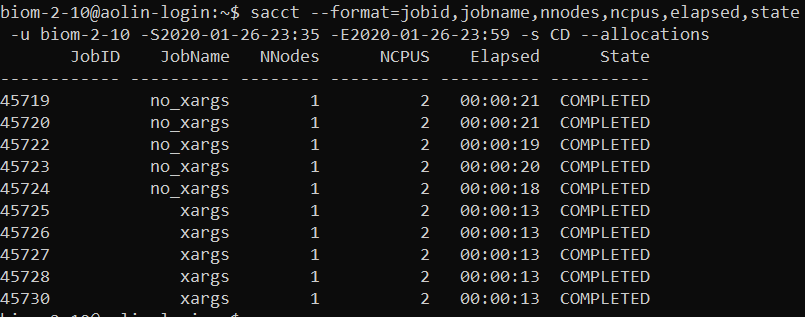
\includegraphics{D:/module5/xargs/runtimes.PNG}

Mean program speed over 5 runs:

\begin{itemize}
\item
  no xargs = 19.8
\item
  xargs = 13
\end{itemize}

Relative performance improvement:

19.8 / 13 \textasciitilde{} 1.52

Using xargs the program was around 1.52 times faster.


\end{document}
